\label{sec:analysis}
This section gives a technical description of the performance and schedulability analysis, as well as a discussion about how the  performance analysis outcomes are interpreted and compared. 

\subsection{Schedulability Analysis}
In our framework, the system schedulability is analyzed as a reachability property using symbolic model checking \cite{Facs2013}. Following our task model, whenever a process misses its deadline it joins immediately the location \ft{DeadlineMiss} (by which the global variable \emph{error} is updated to true). Thus, the schedulability analysis process simply checks whether any task can reach its own \ft{DeadlineMiss} location. Technically, to quantify on all tasks regardless of their identifiers we use the following CTL query supported by Uppaal: \[ \forall []~ \emph{!error}~~~(1)
\]

\subsection{Memory Interference Analysis}
To analyze the delays of access requests performed by a given core, we need to run the execution simulation several times ($X$) each of which lasts for $Y$ time units. The simulation time $Y$ should be greater than the least common multiplier of periods of the tasks mapped to such a core. In fact, the larger $X$ and $Y$ are the more accurate the results will be. To display the average delays of a core $C$, to access L2 and DRAM respectively, in terms of probability distributions we use the following SMC queries: 
\[\begin{array}{ll} E[clk<=Y;X](max:\emph{L2\_ReqDelay}[C]) & (2) \\
                    E[clk<=Y;X](max:\emph{DRAM\_ReqDelay}[C]) & (3) \end{array}
\]

Fig.~\ref{fig:delays} shows the probability distributions of the request delays to L2 and DRAM of a core $C$ where $X=10^3$ and $Y=10^4$. $C$ runs in parallel with another core, each of which serves 2 tasks. Values 2.96 and 4 are the most likely L2 and DRAM access delays respectively because they have the highest probabilities. 

\begin{figure}[ht!]
\centering
\vspace{-5mm}
\caption{L2 and DRAM Request delays.}
\label{fig:delays}
\includegraphics[width=87mm,height=47mm]{Both-delays.pdf}
\end{figure}

																	
\subsection{Utilization Analysis}
To analyze the utilization of cores, we need to run the execution simulation several times ($X$) each of which lasts for $Y$ time units. We accumulate for each simulation the core utilization time via clock \emph{utiliz[cId]}, we consider then the maximum value using the following SMC query:
\[ \begin{array}{ll} \emph{simulate}~ X~ [<=Y]~ {\emph{utiliz}[cId]} &(4) \end{array}\]

\begin{figure}[ht!]
\centering
\vspace{-5mm}
\caption{Simulation of cores utilization.}
\label{fig:core0_utiliz_simul}
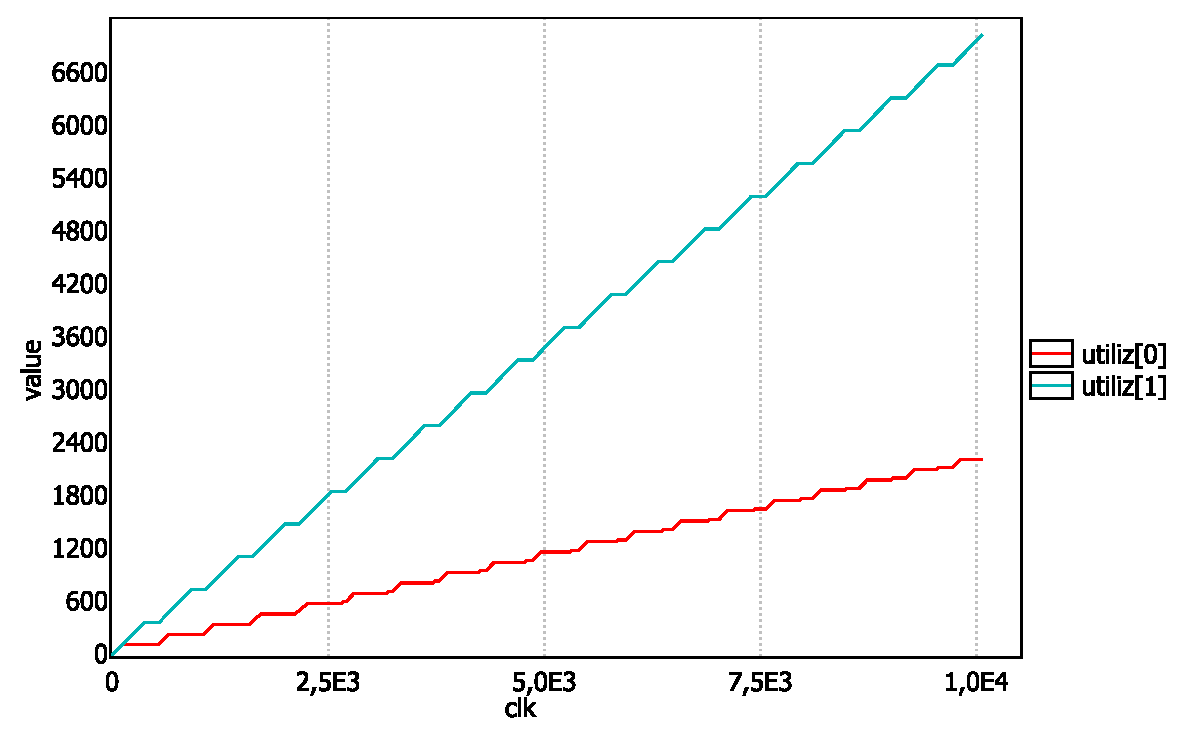
\includegraphics[width=77mm,height=39mm]{Core0_utiliz_Simulation2.eps}
\vspace{-4mm}
\end{figure}

The utilization degree of a given core is then obtained by dividing the accumulated utilization time over the total simulation time $Y$. Fig.~\ref{fig:core0_utiliz_simul} shows the average accumulated utilization time of 2 individual cores ($C_0$ and $C_1$) for 1000 simulations. Each simulation runs for 10000 clock ticks (query (4)). Thus, the utilization of core $C_0$ is $2223/10^4*100=22.2\%$. %The cores utilization can be generated as well in terms of a probability distribution %Similarly, the maximum utilization of a given core can be generated in terms of a probability distribution using the following query: \[\begin{array}{ll} E[clk<=Y;X](max:utiliz[cId]) & (5) \end{array}\]

The fact that read requests are blocking, they contribute majorly in the cores utilization by making cores stalling.  
On the other hand write accesses are not blocking and have a less important impact on the utilization, even though write accesses make the waiting queue longer, which some how might delay other read accesses.

\subsection{Performance Comparison}
We use the multi-objective Pareto frontier to compare the performance of system configurations having different scheduling policies. We emphasize that we compare different configurations of the \textit{same} system, where only scheduling policies vary from a configuration to another. Hence, our framework cannot be used to compare unrelated systems. To perform comparison, one can keep varying scheduling policies, while schedulability and functional requirements are satisfied, until better performance is achieved.   

 

 



